\section{Implementation}
% Exact PVSS scheme choice and parameters (concrete curve, primes, etc.),
% state the complexity.

We implement all on-chain components of the scheme in Solidity and off-chain components in Typescript and Rust.
We use SCRAPE~\cite{pvss_scrape} as the underlying PVSS scheme by adapting the implementation given by Gurkan et al.~\cite{aggregatable_dkg}.
Since SCRAPE relies on Type 3 pairings, our PVSS ciphertext is instantiated using the curve BN254~\cite{bn254}, as at the time of writing only BN254 pairings are available as precompiles on Ethereum.
Similar to the scheme presented by Schoenmakers~\cite{pvss_schoenmakers}, SCRAPE's dealer shares $s$ but the committee recovers $h^s$, where $h$ is the generator of $\mathbb{G}_2$ in BN254.
Therefore, our implmentation of the scheme requires the dealer to encrypt the message with the truncated SHA256 hash of a $h^s$, where $s$ is a randomly generated integer between 0 and the order of BN254.

We also optimize the zkSNARK circuit from Algorithm \ref{alg:snark_circuit} needed to ensure non-malleability.
SCRAPE's instantiation of \textsf{PVSS.verifyDist} allows us to be convinced that $\textsf{PVSS.genDist}(s, \textsf{Cassiopeia}.pks) = c$ just by checking one group element in $c$.
In particular, SCRAPE's ciphertext includes a commitment $F_0 = g^s$.
Since \textsf{PVSS.verifyDist} already checks consistency of $F_0$ with the rest of the ciphertext, we only need to check whether $\log F_0 = s$.
This involves only one BN254 exponentiation inside of Algorithm \ref{alg:snark_circuit} and makes the circuit size constant, allowing proving time to be constant.
To optimize the prover time of the zkSNARK further, we compress the problem instance by first hashing $(c, \mathcal{R}, x, y)$ before passing it into $H$, and instantiate $H$ using Poseidon~\cite{poseidon}, a SNARK friendly hash function.
The primary bottleneck of performance is \textsf{PVSS.verifyDist}, which occurs on chain and has $O(n)$ complexity using SCRAPE, which is the optimal complexity of any PVSS scheme.

% Experimental methodology (Ethereum mainnet, Solidity, give GitHub link / open source license).

% Gas cost VS committee size
We measure the gas cost paid for by the dealer in order to share a secret, which includes verifying the PVSS distribution and the zkSNARK.
\begin{figure}
\caption{Gas cost of \textsf{shareSecret} vs committee size}
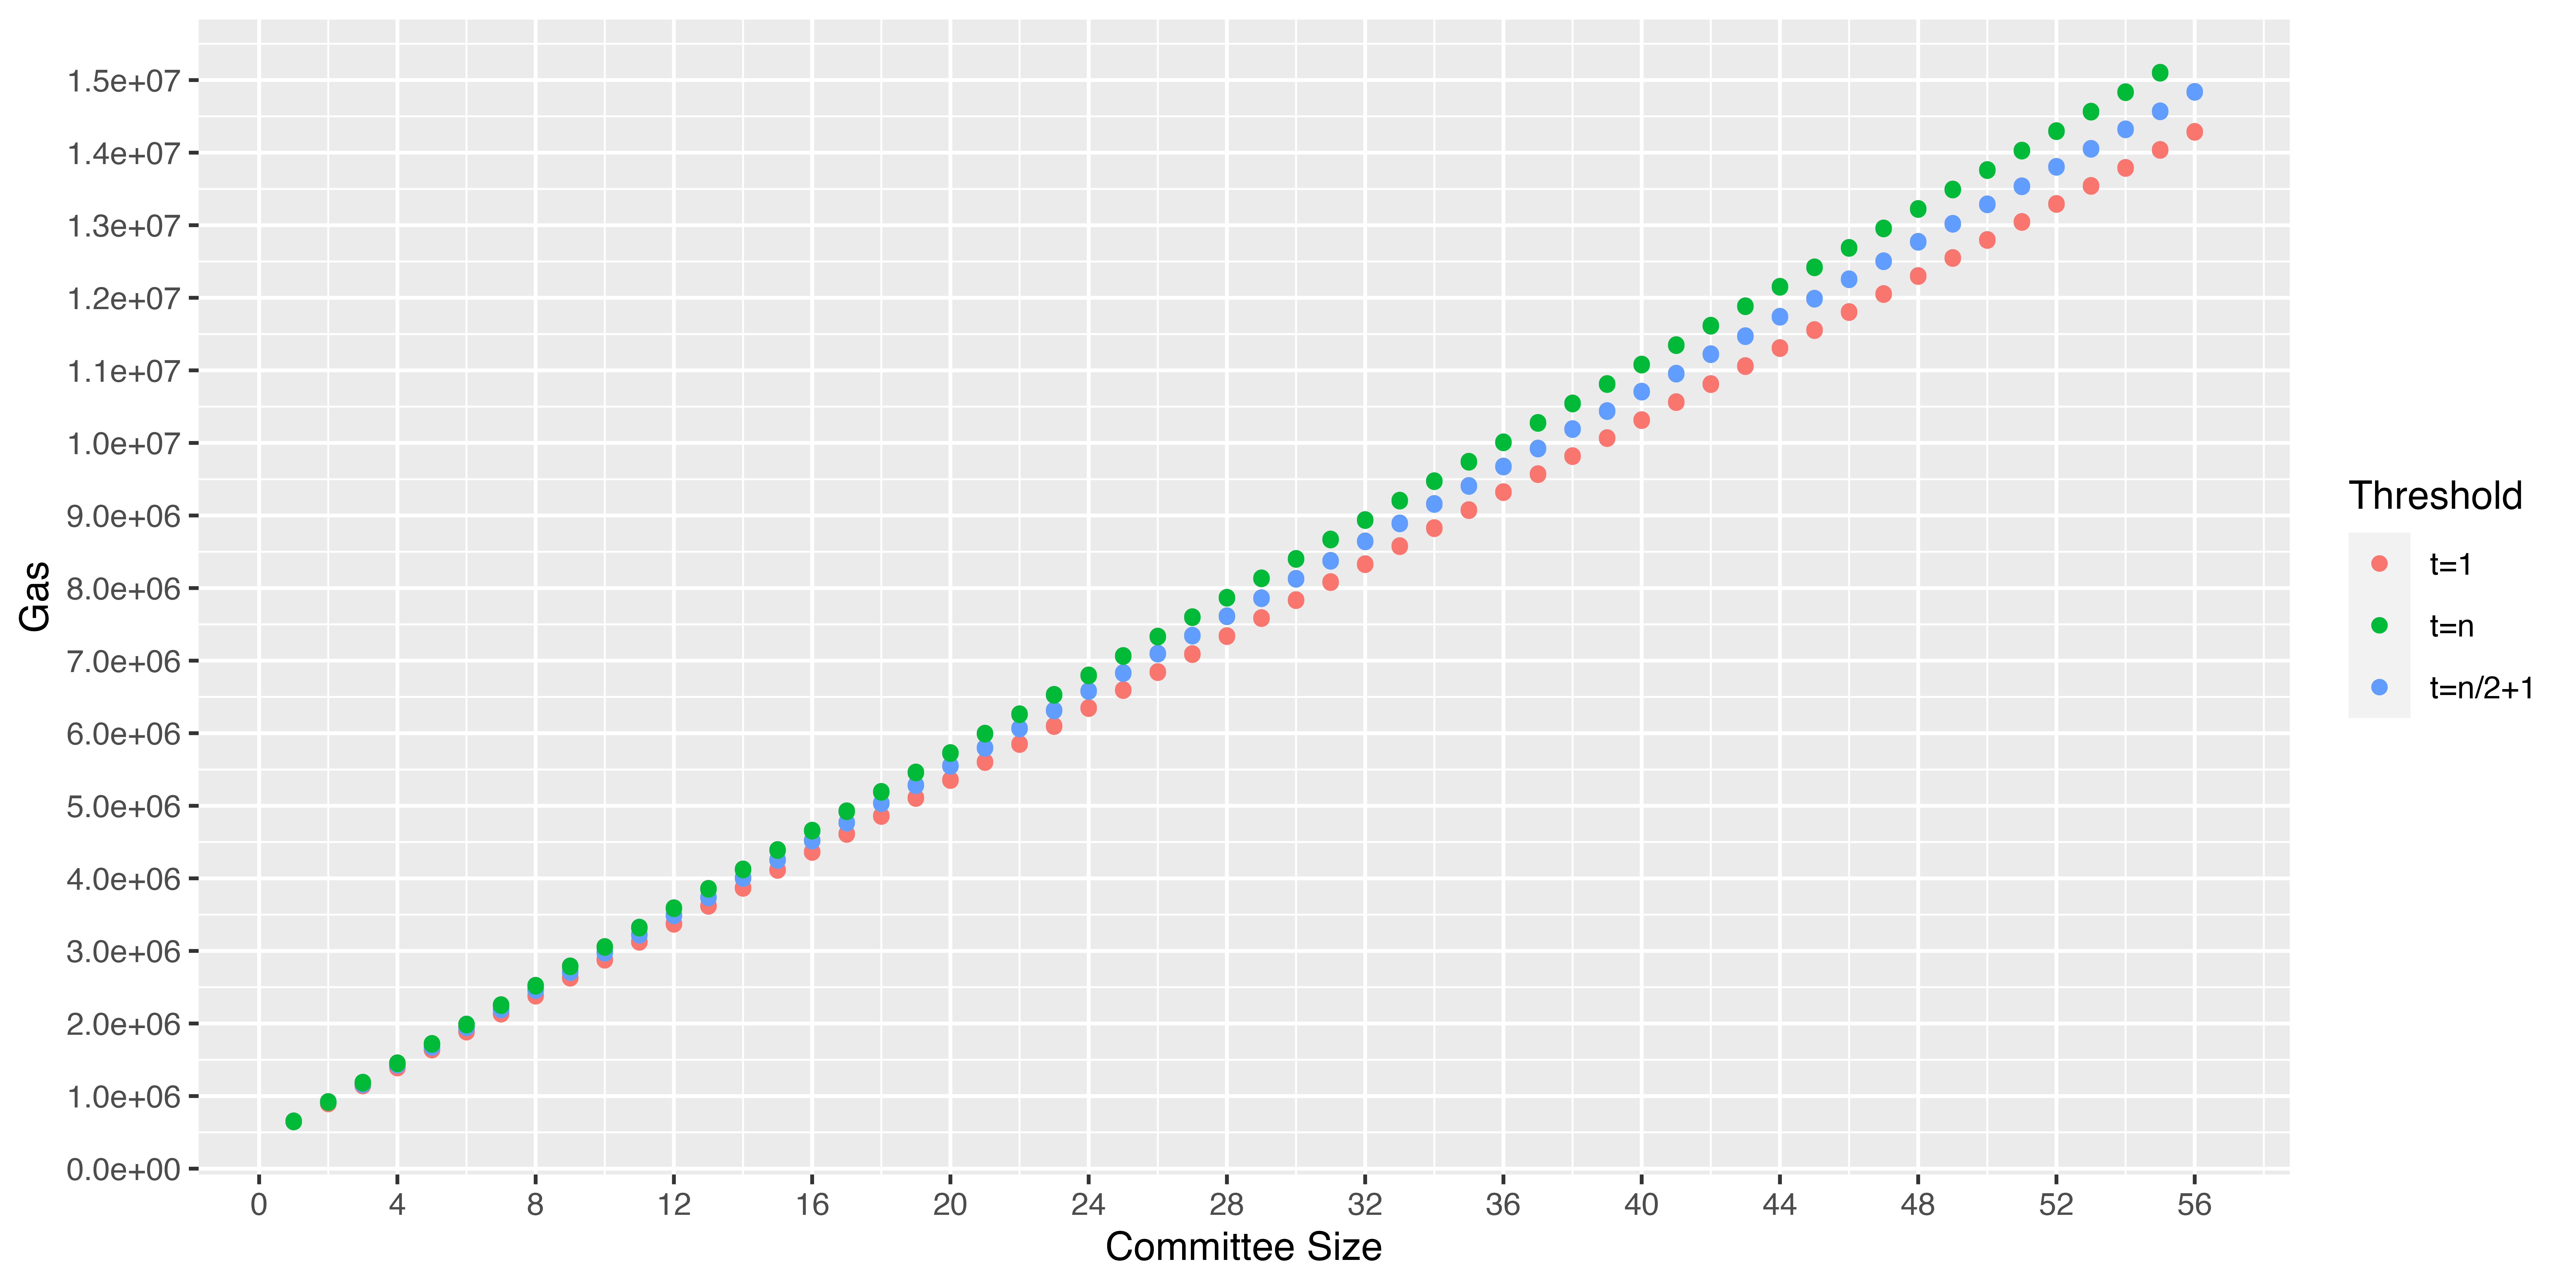
\includegraphics[width=\textwidth]{gas_cost}
\end{figure}

% Offchain computation time VS committee size
% Link to GitHub